% Volume three architecture figures. Independent export only; not book fonts.
\colorlet{MutedBlueFill}{FigureBlueFill}
\colorlet{MutedGreenFill}{FigureGreenFill}
\colorlet{MutedPurple}{FigurePurple}
\colorlet{MutedPurpleFill}{FigurePurpleFill}
\tikzset{
 v3 picture/.style={x=1mm,y=1mm,font=\figurefont\fontsize{8}{10}\selectfont,text=FigureInk,line width=.65pt},
 v3 box/.style={draw=FigureBlue,fill=white,rounded corners=1.8pt,line width=.7pt,inner sep=2.5pt,align=center},
 v3 data/.style={v3 box,fill=FigureBlueFill},
 v3 model/.style={v3 box,draw=FigureGreen,fill=FigureGreenFill},
 v3 output/.style={v3 box,draw=FigureYellow,fill=FigureYellowFill},
 v3 risk/.style={v3 box,draw=FigureRed,fill=FigureRedFill},
 v3 group/.style={draw=FigureBlue,rounded corners=1.8pt,line width=.65pt,inner sep=3mm},
 v3 flow/.style={draw=FigureStroke,line width=.75pt,-{Stealth[length=1.65mm,width=1.05mm]},rounded corners=1pt},
 v3 guide/.style={draw=FigureMuted,line width=.6pt,dashed},
 v3 feedback/.style={v3 flow,draw=FigureGreen,dashed},
 v3 title/.style={draw=none,fill=none,font=\figurefont\fontsize{8}{10}\selectfont,align=center,inner sep=1pt},
 v3 note/.style={draw=none,fill=none,font=\FigureNoteFont\fontsize{7.5}{9.5}\selectfont,text=FigureMuted,align=center,inner sep=1pt},
 v3 label/.style={draw=none,fill=none,font=\figurefont\fontsize{8}{10}\selectfont,align=center,inner sep=1pt},
 v3 wire/.style={draw=FigureMuted,line width=.45pt},
 v3 point/.style={circle,draw=FigureBlue,fill=FigureBlueFill,minimum size=2.3mm,inner sep=0pt,line width=.55pt}
}
% Bring pre-existing native TikZ geometry to the same typography and scale.
\tikzset{
 foundation picture/.append style={font=\figurefont\fontsize{8}{10}\selectfont,line width=.65pt},
 foundation node/.append style={rounded corners=1.8pt,line width=.7pt,font=\figurefont\fontsize{8}{10}\selectfont},
 foundation heading/.append style={draw=none,fill=none,font=\figurefont\fontsize{8}{10}\selectfont},
 foundation note/.append style={draw=none,fill=none,font=\FigureNoteFont\fontsize{7.5}{9.5}\selectfont},
 foundation flow/.append style={line width=.75pt,-{Stealth[length=1.65mm,width=1.05mm]}},
 foundation frame/.append style={rounded corners=1.8pt,line width=.7pt},
 foundation edge label/.append style={draw=none,fill=none,font=\figurefont\fontsize{8}{10}\selectfont}
}
% Official Lucide outline icons, consistently used across diagrams. Size in mm.
\newcommand{\VIcon}[5]{\node[inner sep=0pt] at (#2,#3) {\includegraphics[width=#4mm]{figures/03-foundations/00-shared/tikz/icons/#1-#5.pdf}};}
% A neutral network glyph (not a claim about an actual model architecture).
% Coordinates denote its centre; scale 1 gives 13 x 8 mm.
\newcommand{\VNet}[4]{\begin{scope}[shift={(#1,#2)},scale=#3]
 \foreach \a in {-3,0,3}{\foreach \b in {-3,0,3}{\draw[v3 wire] (-5,\a)--(0,\b);}}
 \foreach \a in {-3,0,3}{\draw[v3 wire] (0,\a)--(5,0);}
 \foreach \a in {-3,0,3}{\draw[draw=#4,fill=#4,line width=.55pt] (-5,\a) circle(.9);\draw[draw=#4,fill=white,line width=.55pt] (0,\a) circle(.9);}
 \draw[draw=#4,fill=#4,line width=.55pt] (5,0) circle(.9);
\end{scope}}
\newcommand{\VDots}[4]{\foreach \k in {0,1,2,3}{\fill[#4] ({#1+2.7*\k},#2) circle(#3);}}
% Feature vector/tensor elements are scientific glyphs, not decorative icons.
\newcommand{\VVector}[4]{\foreach \k in {0,...,4}{\fill[#4,rounded corners=.25pt] ({#1+2.2*\k},#2) rectangle ++(1.5,#3);}}

\newcommand{\SemiSample}[4]{\node[inner sep=0pt] at (#2,#3) {\includegraphics[width=#4mm,height=#4mm,keepaspectratio]{figures/03-foundations/01-basics/tikz/semi-supervised-learning/assets/#1.png}};}
\begin{tikzpicture}[v3 picture]
\path[use as bounding box] (0,0) rectangle (163,70);
\node[v3 title] at (34,66) {少量带标签图像};
\draw[v3 data] (1,38) rectangle (67,62);
\foreach \x/\im/\s in {9/dog/狗,23/cat/猫,37/bird/鸟,51/car/汽车}{
 \SemiSample{\im}{\x}{52}{11}\node[v3 label] at (\x,42) {\s};}
\VDots{59}{51}{.5}{FigureBlue}
\node[v3 title] at (34,29) {大量无标签图像};
\draw[v3 box,draw=FigureGreen,fill=FigureGreenFill] (1,4) rectangle (67,25);
\foreach \x/\im in {9/horse,23/cow,37/sparrow,51/plane}{\SemiSample{\im}{\x}{14.5}{11}}
\VDots{59}{14.5}{.5}{FigureGreen}
\node[v3 output,minimum width=23mm,minimum height=7mm] (super) at (84,53) {监督目标};
\node[v3 data,minimum width=23mm,minimum height=7mm] (struct) at (84,15) {结构信息};
\node[v3 model,minimum width=29mm,minimum height=24mm] (net) at (110,34) {};
\node[v3 title] at (110,59) {共同学习的分类器};\VNet{110}{34}{1.6}{FigureBlue}
\node[v3 output,minimum width=24mm,minimum height=7mm] (out) at (116,9) {预测类别};
\node[v3 title] at (149,51) {新图像};
\node[inner sep=0pt] (new) at (149,34) {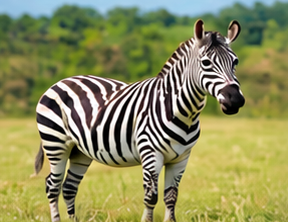
\includegraphics[width=24mm,height=19mm,keepaspectratio]{figures/03-foundations/01-basics/tikz/semi-supervised-learning/assets/zebra.png}};
\draw[v3 flow] (67,53)--(super.west);\draw[v3 flow] (67,15)--(struct.west);
\draw[v3 flow] (super.east)--(99,53)--(99,49)--(104,49)--(104,46);
\draw[v3 flow] (struct.east)--(102,15)--(102,22);
\draw[v3 flow] (new.west)--(net.east);\draw[v3 flow] (net.south)--(110,18)--(116,18)--(out.north);
\end{tikzpicture}
